%Data_to_Computer
\chapter{Getting data to the Computer}
We now have voltage data coming from our Arduino into the computer serial port, and we can see that data with the Arduino serial port monitors. But suppose we want to analyze our data in another program. How would we get the data into Excel or LoggerPro, or even our beloved Python that we learned to use in PH150?

There are lots of ways to do this, but an easy way is to use our Python skills and write a simple code using the Python serial port library. That is what we are going to do in this lab.

\section{How to get Python -- Skip if you have python}

But wait, you might say, I didn't use snakes in PH150. What are you even talking about? Or maybe you got rid of Python because you never thought you would use it again. Whatever the case, Python is another way to make computer code like our Arduino app. Only, this code is designed to work on our computer, itself. This is just what we want for getting the data ready for analysis on our computer. If you already have Python, that is fine, you could skip ahead. If you don't, the next steps show how to get Python on your computer and how to get the Python serial library so you have the commands to read the serial port. Our physics department uses two different distributions of Python. Canopy, and Anaconda. But both work fine. But if you don't have a distribution, I encourage you to try the Anaconda version. Instructions for downloading and installing are given next. 

\subsection{Getting Anaconda Python}

The Anaconda distribution of Python is designed for scientific work (so it has most of the science libraries of functions already installed) It can be found at https://www.continuum.io/downloads. There is an install link for Windows, Mac, and Linux. Choose the one for your operating system\footnote{If you have a Linux computer, it is likely that you will want to actually see if Anaconda is in your distribution's repository. If you are not a Linux user and you have no idea what that means you can ignore it.}

When you click on the green download button it will download an executable file. Meanwhile the website tries to get you to subscribe, and offers you the opportunity to code with Anaconda in the cloud. I encourage you to ignore these opportunities and to just use the executable file to install python. In windows it looks like this 

\begin{figure}[h!]
	\centering
	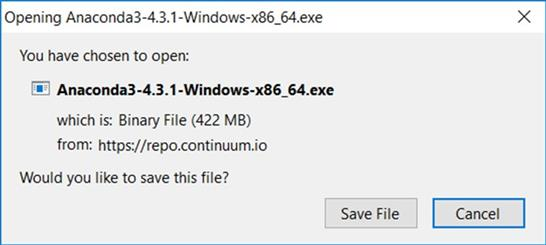
\includegraphics[width=4.0in,height=1.9in]{PH4CAU23}
\end{figure}

Choose ``Save File'' and when the file is downloaded open it to start the installation. You should see something like this: 

\begin{figure}[h!]
	\centering
	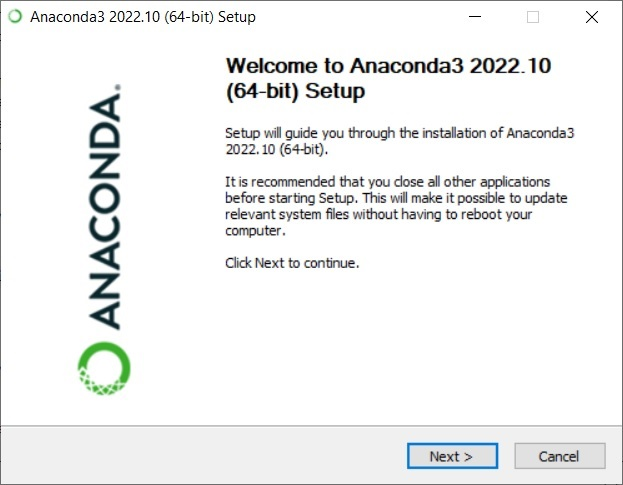
\includegraphics[width=3.1502in,height=2.2361in]{PH4CAU24}
\end{figure}

Choose ``Next'' and follow the installation instructions. If all goes well, you should have a new set of apps. Here is what mine looked like on my Windows 10 computer. 

\begin{figure}[h!]
	\centering
	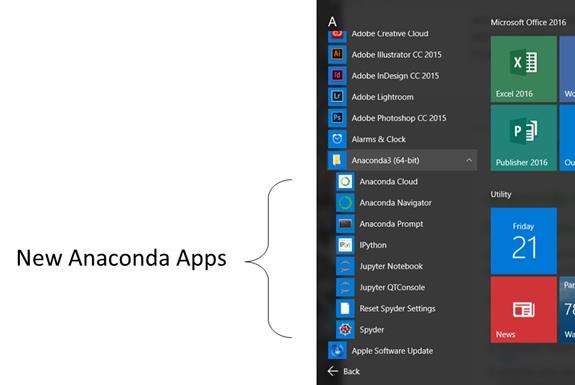
\includegraphics[width=3.8369in,height=2.2448in]{PH4CAU25}
\end{figure}

The list of the apps has an app called Spyder. Let's launch it to see what it does.

\begin{figure}[h!]
	\centering
	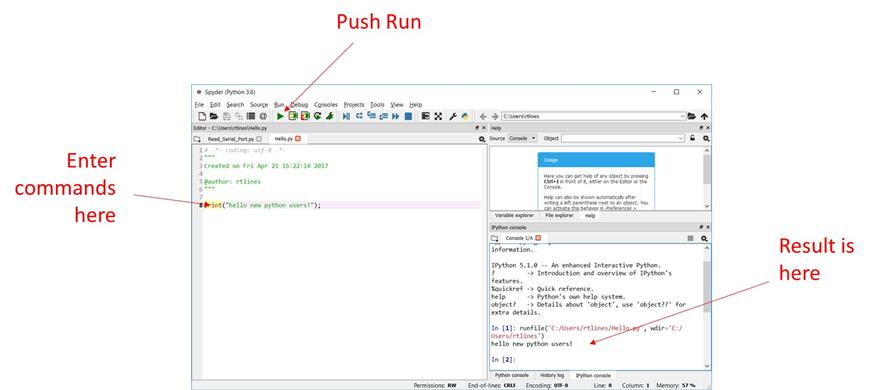
\includegraphics[width=5.655in,height=2.4898in]{PH4CAU26}
\end{figure}

What we get is something like the Arduino program that we have been using to write Arduino sketches. Spyder is a place to write and run Python commands. Only this time there is no checking and uploading the code, because the Python code will run on our computer, not on an Arduino.

In the figure above, the command just says to print ``hello new python users!'' and that is all. When it runs, it prints our message on the small window to the right. But of course Python
can do much more than print silly messages in little windows. We will have our Python system read a serial port and save our data to a file. But we need an additional piece of Python to do this. We need functions that can handle serial ports. These functions are already written by someone, and put together in a package called a \textquotedblleft library.\textquotedblright\
But this library isn't included in what we have downloaded. So we need to fix this next.

\subsection{Getting the PySerial library for Anaconda -- Don't skip this}

Now that we have Python, we need to enhance it with the PySerial library so that we can read our data from the computer serial port. If you have installed the Anaconda package as your Python distribution, follow along here. If you have a different distribution of python, ask your instructor for help.

We will use the Anaconda prompt to get the PySerial library. The Anaconda prompt is an app that let's us modify the Python libraries that we have installed. The Anaconda prompt is found in the list of apps that were installed in Anaconda. If you are using Windows, you might find it in your app list like this.

\begin{figure}[h!]
	\centering
	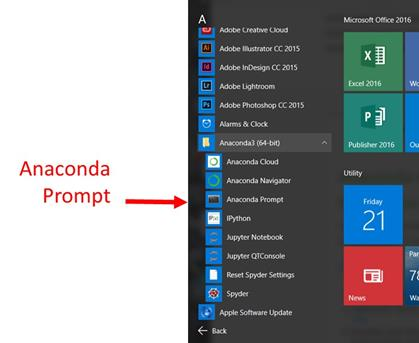
\includegraphics[width=3.5293in,height=2.8928in]{PH4CAU27}
\end{figure}

Once you launch the Anaconda prompt it just looks like a big black box. 

\begin{figure}[h!]
	\centering
	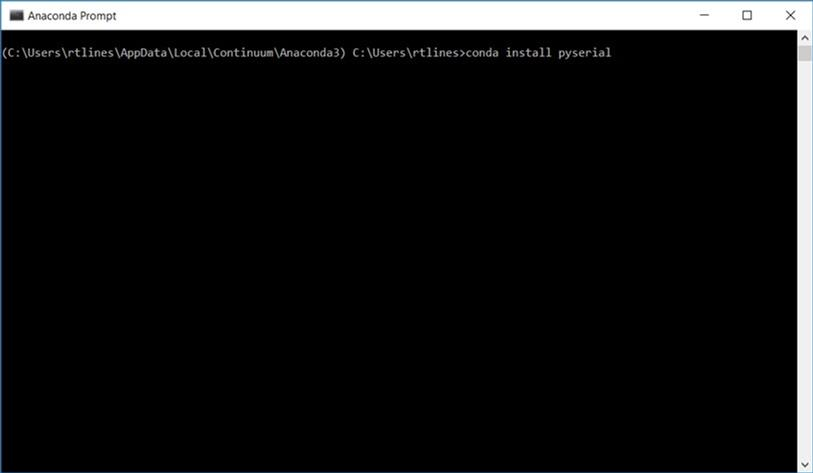
\includegraphics[width=2.2831in,height=1.5796in]{PH4CAU28}
\end{figure}

We can type commands in that box that will modify the Anaconda Python programs that we installed. In our case we want to type in the command \texttt{conda install pyserial}.

\begin{figure}[h!]
	\centering
	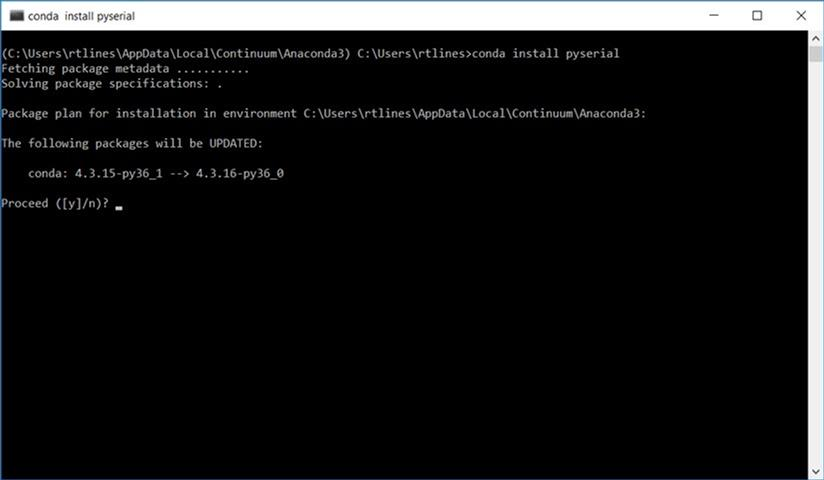
\includegraphics[width=4.2851in,height=2.501in]{PH4CAU29}
\end{figure}

Notice that the Anaconda prompt app responds to our command. What it responds will depend on your computer and your Python distribution. You need a network connection to install new libraries, so if you get an error, you may just not be connected to a network.

\begin{figure}[h!]
	\centering
	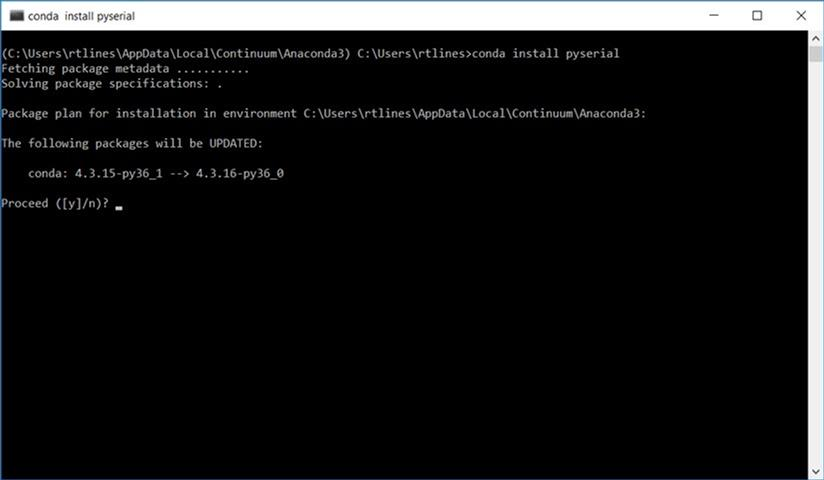
\includegraphics[width=4.2851in,height=2.501in]{PH4CAU2A}
\end{figure}

If you already have PySerial installed, you will be told so, or asked if you wish to update it if an update is available. If you don't have PySerial, it will ask you if you want to install it. Answer ``yes'' and PySerial will be installed. If any error messages are generated, ask for help from your instructor. Hopefully you will see a happy end result like this 

\begin{figure}[h!]
	\centering
	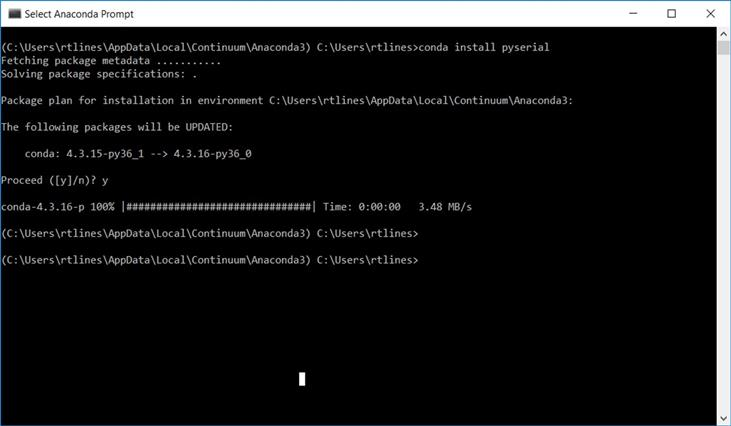
\includegraphics[width=4.2851in,height=2.501in]{PH4CAU2B}
\end{figure}

and you will be all ready to start writing code to get data from the serial port.


\section{Getting data from the Arduino}

It might help to know how a serial port works. The serial port in the computer takes in data from the serial cable. It stores the data in a temporary place in memory called a \emph{buffer}. Whatever data comes into the port goes into that memory location.

\begin{figure}[h!]
	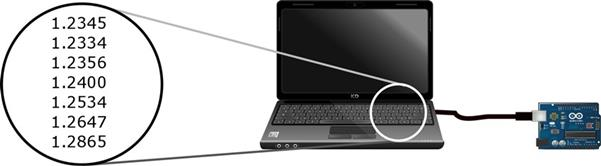
\includegraphics[width=4.5826in,height=1.2791in]{PH4CAV2K}
\end{figure}

Suppose that we set up our Arduino to send data to the port. The Arduino sends data every few milliseconds. But, suppose we only want data every few seconds. We only want some of the data that the Arduino has sent. 

\begin{figure}[h!]
	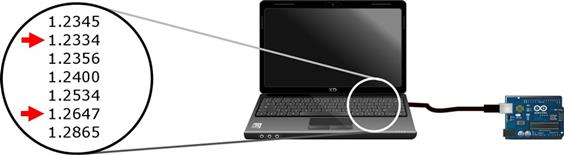
\includegraphics[width=4.7444in,height=1.3188in]{PH4CAV2L}
\end{figure}

The computer has placed every data point sent by the Arduino into it's buffer, and the buffer must be read in sequence. You can't skip data values. But this is just what we want to do, skip some data values and take a value every few seconds. A way to do this is to continuously read in data, but only store it every few seconds. We will use this technique in the code that follows.

Just for fun, let's think of an actual data collection. Suppose we want to measure a voltage from our Arduino, but we want to measure it many times, each time five seconds apart. This way we are looking at how the voltage changes over time. We might want $10$ total measurements.

You might be an expert Python programmer, and if so you can probably see how to write this code. If so, go ahead and do so. But if not, let me introduce some of the Python code elements we will need, and then give an example code. 

The first new code piece is making files for our data. We create a file with a line like this (see the actual code below):
\vspace{.1in}

\begin{python}
	fileObject=open("C:\\Users\\rtlines\\Documents\\data.txt","w")	
\end{python}
\vspace{.1in}

The ``fileObject'' is a variable that contains all the file information like the path and file name. It is way easier to type than to include all that information each time we use a file. So we will use fileObject variables. In the code below I named the fileObject variable ``dataFile.'' Of course, you will have to choose your own path where you will place the data file (you can't use mine, because you don't have my computer!) and you will need to choose your own file name. Notice the weird double slashes $\backslash$$\backslash$.'' These are a Python thing and you probably need to write the path this way.

The other new code piece is dealing with serial ports. Like with our Arduino code, we have to set up the serial port. We do that with the line like the this (also see the actual code below).

\vspace{.1in}
\begin{python}
	ser=serial.Serial('COM6', baudrate = 9600, timeout=1)
\end{python}
\vspace{.1in}

Note that when I was using this code my Arduino was in COM6. But that might not be true for you. Use the Arduino app to find out where your Arduino is connected. 

\begin{figure}[h!]
	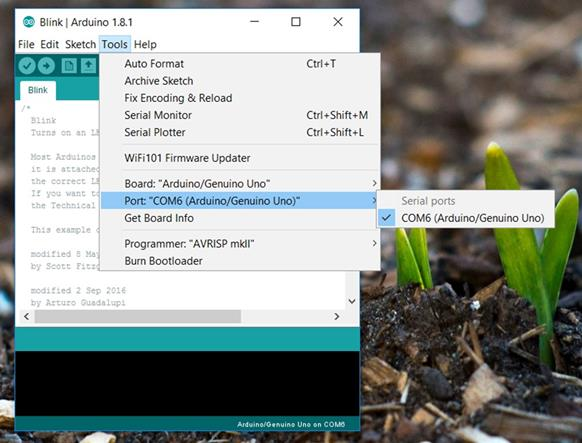
\includegraphics[width=4.8957in,height=3.7308in]{PH4CAV2M}
\end{figure}

The COM port number must match. This looks a little uglier on a Mac, but is much the same. Once the serial port is set up, a line like 

\vspace{.1in}
\begin{python}
	arduinoData=ser.readline().decode('ascii')
\end{python}
\vspace{.1in}

\noindent will read data from the serial port and ``decode it'' so that it is text that we can use in another program. The rest of the example code writes the data point to a file. I have the Areduino code calculate a value in miliseconds for when the data points are taken. This is passed along with the voltage through the serial port. From this we could calculate the time since the beginning of our data collection (we might just need that in a future lab). This time in milliseconds is output into the file as well.

We are going to want a name for the amount of time in between data points. In the example code, the amount of time to delay in between data points is named \pyth{sleeptime} and the number of data points is named \pyth{N}.

At the end of the program we close the file

\vspace{.1in}
\begin{python}
	fileObject.close()
\end{python}

\begin{python}
	ser.close()
\end{python}
\vspace{.1in}

\noindent so that it will be ready to use next time. Your complete code might look
something like this.

%%%%%%%%%%%%%%%%%%%%%%%%%%%%%%%%%%%%%%%%%%%%%%%%%%%%%%%%%%%%%%%%%%%%%%%%
% code link here for download
%\href{https://dtoliphant.github.io/PH250Manual/Code/Data2Computer_PythonSide_Win.py}{Download here}
\href{https://raw.githubusercontent.com/rtlines/IntermediateLabPH250/main/Code/Data2Computer_PythonSide_Win.py}{Download here}
%%%%%%%%%%%%%%%%%%%%%%%%%%%%%%%%%%%%%%%%%%%%%%%%%%%%%%%%%%%%%%%%%%%%%%%%
\inputpython{Code/Data2Computer_PythonSide_Win.py}{0}{10000}


Make sure you understand what each line does. Discuss each line with a group member or with the instructor. Python code runs one line at a time. That is different than our Arduino code that must be checked and translated before it goes to the Arduino. Errors in Python code show up as the code runs. If you use the Spyder IDE, the errors show up in the little output box to the
right. If you use Canopy they show up in the lower box of the editor. 

I modified my simple voltmeter to give the time that the data was taken and to send both the time and the voltage to the serial port. Here is my sketch (remember since it is a simple voltmeter it can only handle $0\unit{V}$ to $+5\unit{V}.$)

%%%%%%%%%%%%%%%%%%%%%%%%%%%%%%%%%%%%%%%%%%%%%%%%%%%%%%%%%%%%%%%%%%%%%%%%
% code link here for download
%\href{https://dtoliphant.github.io/PH250Manual/Code/Data2Computer_ArduinoSide_Win.ino}{Download here}
\href{https://raw.githubusercontent.com/rtlines/IntermediateLabPH250/main/Code/Data2Computer_ArduinoSide_Win.ino}{Download here}
%%%%%%%%%%%%%%%%%%%%%%%%%%%%%%%%%%%%%%%%%%%%%%%%%%%%%%%%%%%%%%%%%%%%%%%%%%%%
\lstinputlisting[language=Arduino]{Code/Data2Computer_ArduinoSide_Win.ino}


You can't use the Arduino serial monitor and get data from the serial port using Python at the same time. So turn off the serial monitor if it is running.

Now that we have our data in a file, we can analyze it. You might try opening the file in Excel or another spreadsheet program and plotting the data. If you know Python, you could add more code to plot the data right in the code that takes it from the serial port. But, if you are new to Python, you could plot the data in something like a Excel or LoggerPro. Ask for help if you don't know how to do this. We will plot data in future labs.

\section{Getting Pyserial if you have a Mac -- skip if you don't have a Mac}

Of course, we have a diversity of computers on campus. The instructions I gave above are for a PC type computer.

\subsection{Anaconda Mac Users 4.1.2}

Go to the Anaconda Prompt and type in: \textit{conda install -c anaconda pyserial}. This will install pyserial -v3.4.

%Note to Brother Lines: The rest of the steps %for Anaconda should be the same as the %Microsoft steps.

If this does not work for some reason, try going to the Anaconda Navigator, on the left hand side, click Environments. Next, on the right hand side, change the drop-down from Installed to Not Installed. Then enter serial in the search box. Check the box for pyserial and click the Apply button. If you have Spyder running, then relaunch Spyder.

% I didn't get to try this since I don't have Anaconda but I did look into it for Macs. The second option looks like the method that is to be used at least that is the method we have used in the past. 

\subsection{Canopy Mac Users 4.2.1 -- skip if you don't have Canopy}

The steps are the same as the Microsoft Version.

\subsection{Manually install pyserial through the terminal on a Mac. Codingin emacs/VI}

This is kind of a ``last resort'' approach, so only try this if the other methods above fail.

\begin{enumerate}
	\item First, go to \textit{https://pypi.python.org/pypi/pyserial} and download \textit{pyserial-3.4.tar.gz} or the version that correlates with the version of python you are using. If you are using python 2 then instead of 3.4, you should look for a file that starts with 2.x; however, if you are using python 3 then 3.4 is the correct version of pyserial you are looking for (but please consider using python 3.x!).

	\item Be sure that you downloaded to your Downloads folder.

	\item Go to your search bar and type in \textit{terminal} and open that application.

	\item Type into the command line \textit{cd Downloads} then press enter.

	\item Next, type in \textit{tar -xzf pyserial-3.4.tar.gz} then press enter. Type in \textit{cd pyserial-3.4}, press enter

	\item Then type in \textit{sudo python3 setup.py install}. 

	\item If you are using python 2 then only type in \textit{python} where it says \textit{python3}.
\end{enumerate}

\noindent After that you are ready to use the serial library in python.

\subsection{Mac Pathway and Port Notation -- Skip if you don't have a Mac}

Mac computers list paths to files differently than PC computers.

\subsubsection{Mac Pathway}

In fact, Mac computers don't make file locations obvious to users at all! But our python code needs to know where to put the files we build, so we will need to understand how to do this.

On the line of code that starts with \textit{dataFile} you will replace it with \textit{dataFile = open(\textquotedblleft /Users/rtlines/Documents/data.csv",\textquotedblleft w")}. This is in the form of /Users/username/folder name/(optional if you have a folder within
the previous folder) folder name/file name + extension (e.g. .csv or .txt).

You can find your username by going to your download folder then right click on any file in there and select \textbf{Get Info}. Next make sure that the arrow to the left of \textit{General} is pointing down. Once it is pointing down look at the line that reads, \textbf{Where: Macintosh HD $\rightarrow $ Users $\rightarrow $ your username will be here $\rightarrow $ Downloads}.

\subsubsection{Mac Port}

Mac computers also deal with serial ports differently. So we need to change that next line of code after the dataFile line that begins with \textit{ser = serial...}. The line of code will need look something like \textit{ser = serial.Serial(`/dev/cu.usbmodem1411', baudrate = 9600, timeout = 1)}. However, yours may vary slightly by a different usbmodem number. To find out
what to place between the apostrophes is by going to your arduino code, click on \textbf{Tools}, scroll down to \textbf{Port} and write down what is written there minus what is in the parenthesis.

\subsection{Mac version of the python code}

%%%%%%%%%%%%%%%%%%%%%%%%%%%%%%%%%%%%%%%%%%%%%%%%%%%%%%%%%%%%%%%%%%%%%%%%
% code link here for download
%\href{https://dtoliphant.github.io/PH250Manual/Code/Data2Computer_PythonSide_Mac.py}{Download here}
\href{https://raw.githubusercontent.com/rtlines/IntermediateLabPH250/main/Code/Data2Computer_PythonSide_Mac.py}{Download here}
%%%%%%%%%%%%%%%%%%%%%%%%%%%%%%%%%%%%%%%%%%%%%%%%%%%%%%%%%%%%%%%%%%%%%%%%
\inputpython{Code/Data2Computer_PythonSide_Mac.py}{0}{10000}

Make sure you understand each line of this code. It is a little fancy in that it tries to check to make sure the SD card file is working properly and warns you if something is wrong. But most of the code is comments. So don't be discouraged by the length.

\section{Lab Assignment -- Really don't skip}

\begin{enumerate}
\item Finish any part of the last lab that you haven't done.

\item Using Python, Save Arduino data to a file on your computer

	\begin{enumerate}
	\item Wire up a simple voltmeter and load its sketch. Build a simple circuit to test like we did back in section (\ref{Voltage Measurement with Meter}). Start your Arduino and check to make sure voltages are going to the serial port by looking at the serial monitor or plotter.
	
	\item Check with your group members to make sure their simple voltmeters are working. Help if they are not.
	
	\item Start your Python system (Spyder or Canopy if you are following the instructions given above) and write the program to read the serial port and save the data to a file.
	
	\item Close the serial monitor and/or serial plotter. Then run your Python code. Check to make sure that the file of data is written properly. The voltages written in the file should match what your power supply and circuit provided.
	
	\item Make sure you save this program and record what you did in your lab notebook.
	
	\item Make sure your lab group members all have Python programs that run and save data correctly. Help if they do not.
	\end{enumerate}

\end{enumerate}
